\section{Analyseklasser}
For at analyseklasserne kan udarbejdes, foretages en analyse ud fra systembeskrivelsen, use case og funktionaliteter til at identificere substantiver og verber. Dette gøres for at sikre, at alle funktionaliteter indgår i design af klassediagrammer. Substantiver og verber fra analysen fremgår af \autoref{tab:subverb}.

\begin{table}[H]
\centering
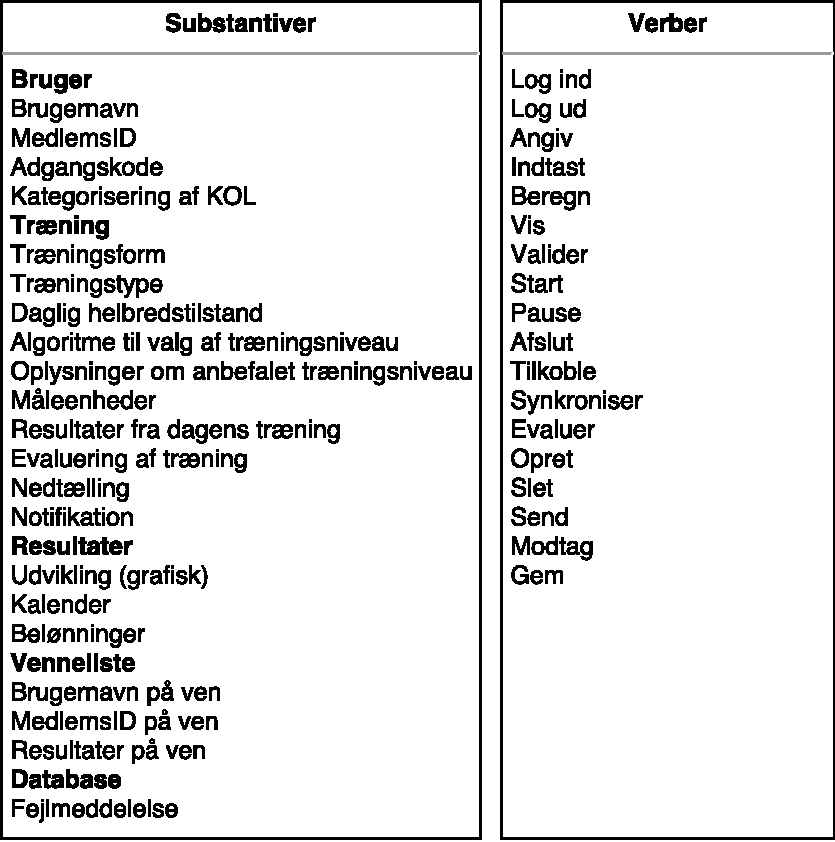
\includegraphics[width=0.7\textwidth]{figures/aktivitetsdiagram/substantiveverber}
\caption{Substantiver og verber identificeret ved analyse af systembeskrivelse, use case samt funktionaliteter.}
\label{tab:subverb}
\end{table}

\noindent
De fremhævede substantiver, brugeroplysninger, tilpasning af træningsniveau, træning, resultater, venneliste og database, identificeres som klasser. Under hver klasse fremgår deres tilhørende attributter, der beskriver den overordnede klasse. Verberne betegner de metoder, der kan tilgås i de forskellige klasser. 

Efter substantiver og verber er identificeret inddeles disse i analyseklasser og opdeles i stereotyperne, entity og control. Dette kan ses af \autoref{fig:analyseklasse}. 

\begin{figure}[H]
\centering
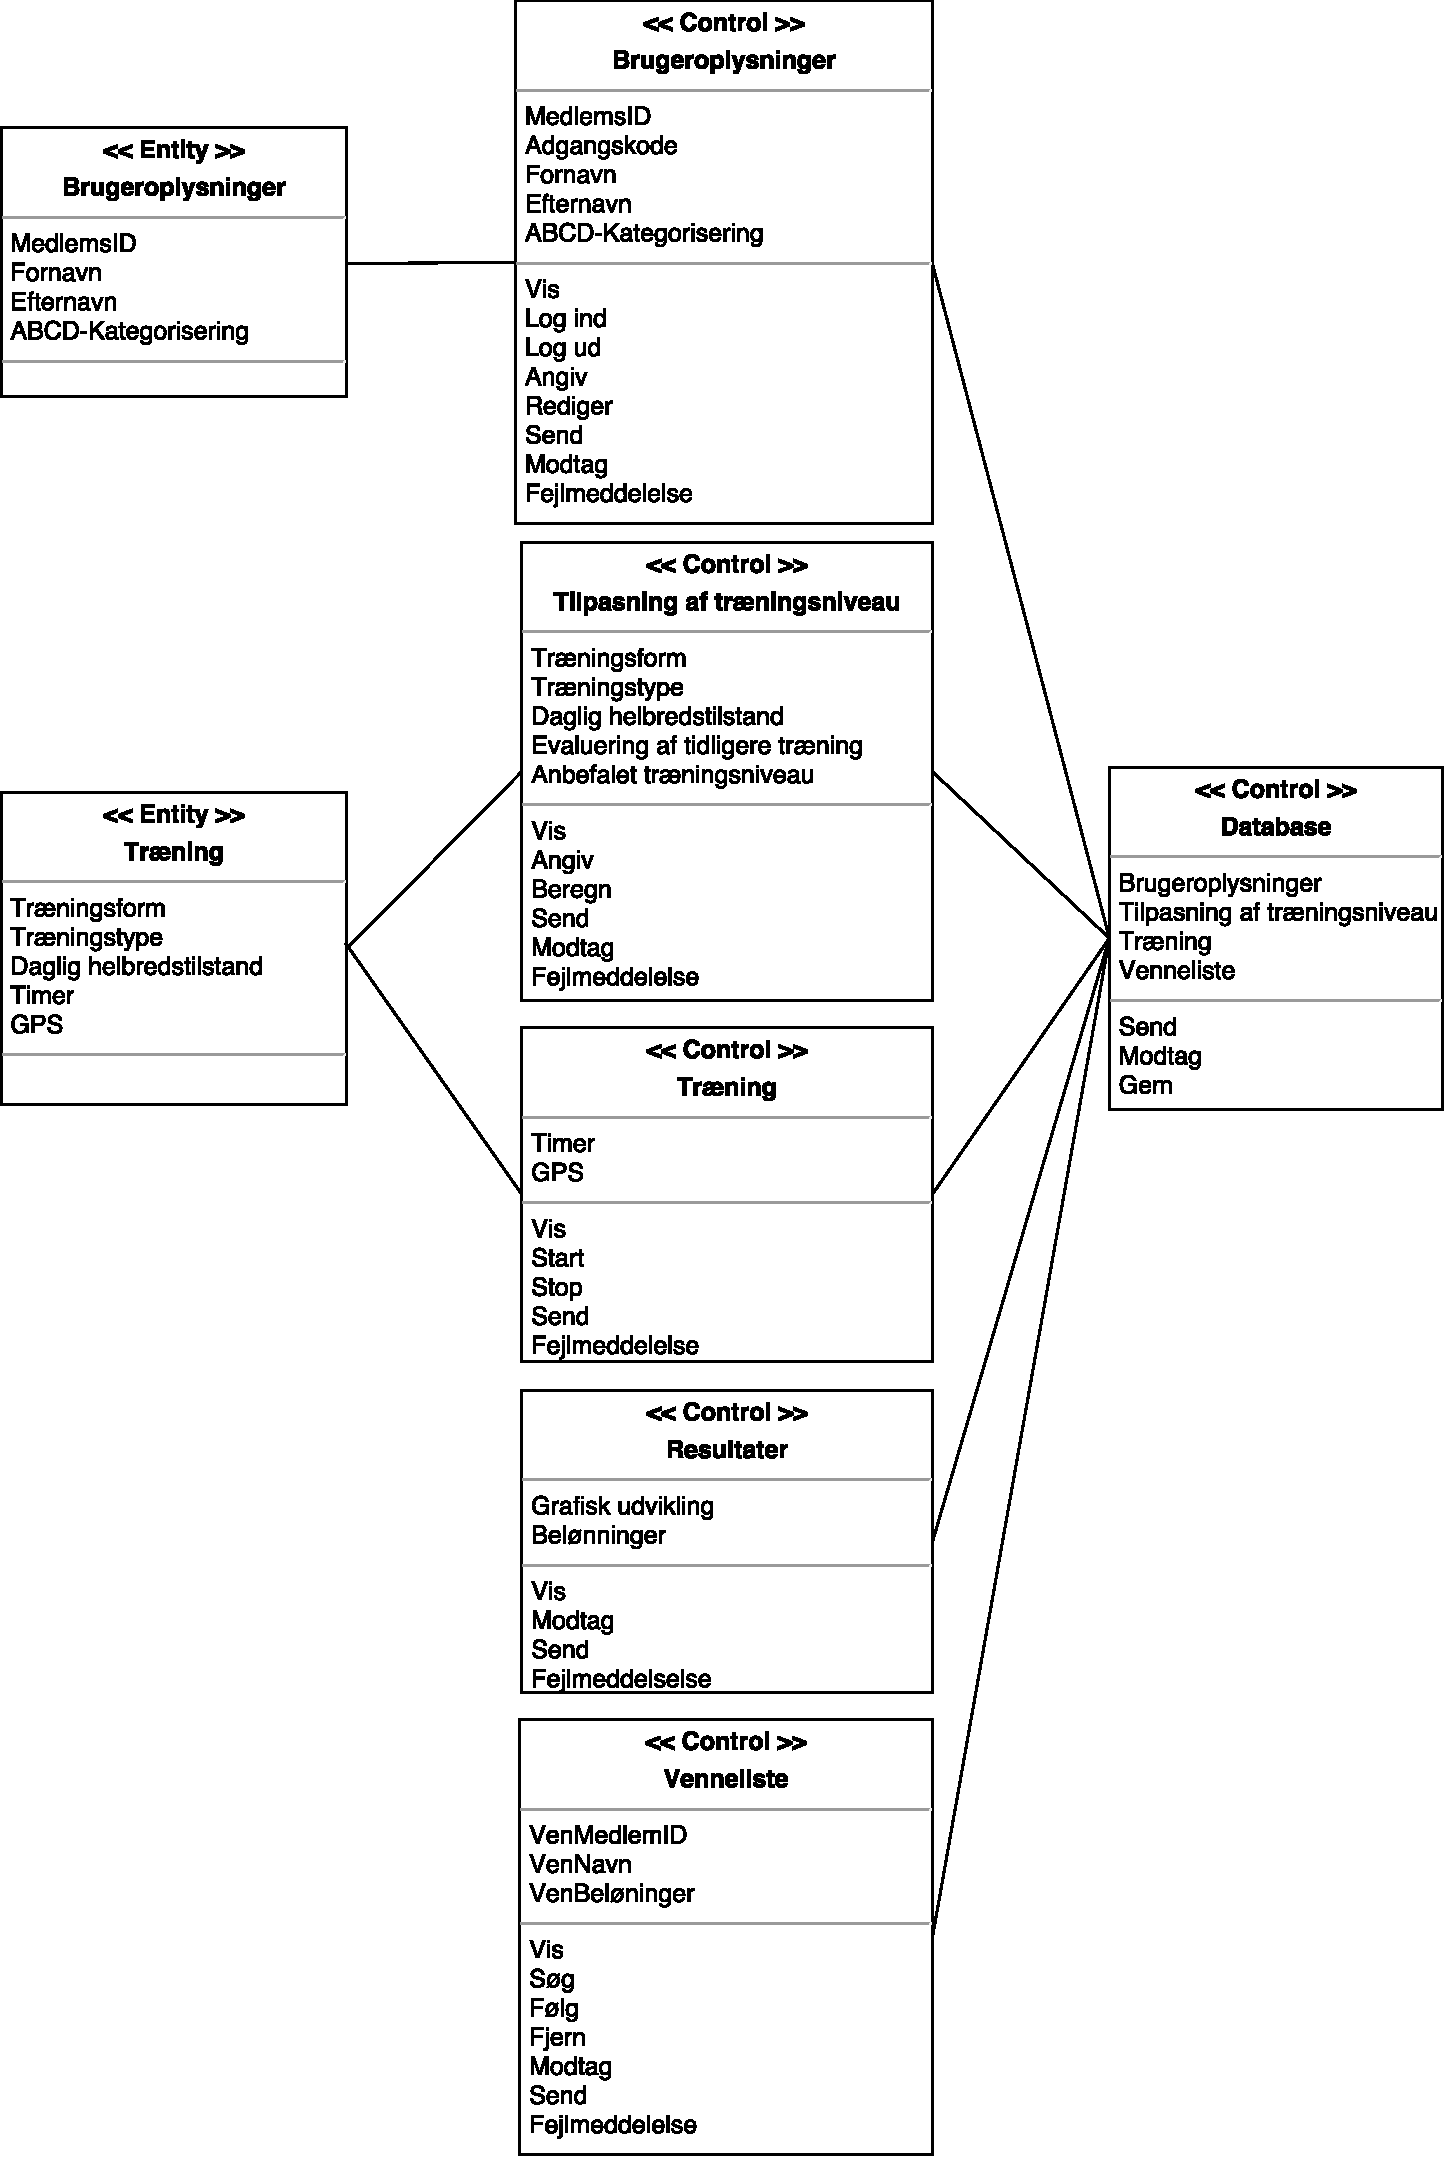
\includegraphics[width=0.7\textwidth]{figures/aktivitetsdiagram/analyseklasser}
\caption{Analyseklasser udarbejdet ud fra de identificerede substantiver og verber.}
\label{fig:analyseklasse}
\end{figure}

\noindent
Af \autoref{fig:analyseklasse} fremgår relationen mellem klasserne og deres tilhørende attributter samt metoder. Controlklasserne indeholder metoderne, der skal udføres når denne tilgås, hvorimod entityklasserne har til formål at lagre data. \textit{Brugeroplysninger} og \textit{Træning} er defineret som entityklasser med tilhørende controlklasser. Entityklassen \textit{Træning} har yderligere controlklassen \textit{Tilpasning af træningsniveau}, da informationer fra denne ligeledes gemmes i denne entity. Derudover er opstillet tre controlklasser, herunder \textit{Resultater},\textit{Venneliste} og \textit{Database}. Klassen, \textit{Database}, tilgås fra samtligt controlklasser, da formålet med denne klasse er at kommunikere med databasen. 